\documentclass[10pt,a4paper]{article}
\usepackage[T1]{fontenc}
\usepackage[utf8]{inputenc}
\usepackage{amsmath, amssymb, amsthm, thmtools, amsfonts, mathtools}
\usepackage{nicefrac}
\usepackage{calc}
\usepackage[pdftex, hyperindex, plainpages=false]{hyperref}
\usepackage[nameinlink]{cleveref} %load before classicthesis (clash)
%\usepackage[nochapters,pdfspacing]{classicthesis}
\usepackage{siunitx}
\usepackage[siunitx]{circuitikz}

\usepackage[a4paper]{geometry}
\usepackage{float}
\usepackage{mdframed}
\usepackage{titling}
\usepackage{booktabs}
\usepackage{graphicx}
\usepackage{caption, subcaption}
\usepackage{xcolor}
\usepackage[italian]{babel}
\usepackage{pgfplots}
\usepackage{listings}
%\usepackage{lmodern}
\usepackage{url}
\usepackage{enumitem}
\usepackage{tikz} %loads after classicthesis (xcolor incompat)

% lets graphicx know path where figures to be included are found
\graphicspath{{../figs/}}
\makeatletter
\def\input@path{{../figs/}}
%or: \def\input@path{{/path/to/folder/}{/path/to/other/folder/}}
\makeatother

% tikz pgf plots setup
\usepgfplotslibrary{external}
\pgfplotsset{compat=1.15}
%\tikzexternalize

% spaces and significant digits/figures for measurements
\sisetup{free-standing-units, space-before-unit, number-unit-product = \;,
scientific-notation = false, round-mode = figures, round-precision = 1,}

% turns all (hyperlinked) references black [default is blue]
\hypersetup{
	linktoc=all,
	colorlinks=true,
	linkcolor=black
}

% code listings config
%\lstset{
%language=Python,
%basicstyle=\ttfamily,
%columns=fullflexible,
%keepspaces=true,
%}

% mdframed (for boxed text) configuration
\mdfsetup{linewidth=0.6pt}

% Default fixed font does not support bold face
\DeclareFixedFont{\ttb}{T1}{txtt}{bx}{n}{12} % for bold
\DeclareFixedFont{\ttm}{T1}{txtt}{m}{n}{12}  % for normal

% Custom colors
\usepackage{color}
\definecolor{deepblue}{rgb}{0,0,0.5}
\definecolor{deepred}{rgb}{0.6,0,0}
\definecolor{deepgreen}{rgb}{0,0.5,0}

% Commands 
\newcommand{\executeiffilenewer}[3]{%
	\ifnum\pdfstrcmp{\pdffilemoddate{#1}}%
		{\pdffilemoddate{#2}}>0%
	{\immediate\write18{#3}}\fi%
}
% input .svg --> .pdf_tex graphs
%\newcommand{\includesvg}[1]{%
%	\executeiffilenewer{#1.svg}{#1.pdf}%
%	{inkscape -z -D --file=#1.svg %
%	--export-pdf=#1.pdf --export-latex}%
%	\input{#1.pdf_tex}%
%}
% Thanks UniPi's Department of Physics E. Fermi
\newcommand{\thanksdf}{(\thanks{Dipartimento di Fisica E.~Fermi,%
Universit\`a di Pisa - Pisa, Italy.}\;)}

% hyperlink to email address
\newcommand{\mail}[1]{\href{mailto:#1}{\textsf{#1}}}

\geometry{left=2cm, right=2cm, top=2cm, bottom=2cm}
\newcommand{\rem}[1]{[\emph{#1}]}
\newcommand{\exn}{\phantom{xxx}}

% lets graphicx know path where figures to be included are found
\graphicspath{{../figs/}}

\author{Gruppo 1.AC \\ Matteo Rossi, Bernardo Tomelleri}
\title{Es01A: Uso dello strumento Analog Discovery 2.}
\begin{document}
\date{\today}
\maketitle

\setcounter{section}{1}

\section{Utilizzo del canale di alimentazione e del multimetro}

\subsection*{2.d Accensione diodo}

La tensione di alimentazione \`e stata variata nell'intervallo tra
$0.5\,\mathrm{V}$ e $5\,\mathrm{V}$


Si osserva che la luminosit\`a del diodo è proporzionale alla tensione
erogata dal generatore, una volta superata una tensione di soglia per cui
il LED inizia a emettere luce di intensità osservabile. La tensione di soglia
varia per i diversi colori; in particolare $V_{\mathrm{thr}}$ risulta
proporzionale alla frequenza del colore di luce emessa. Dunque
rosso $<$ giallo $<$ verde $<$ blu.

\subsection*{2.e Misura tensione}
Utilizzando il multimetro si misura la tensione ai capi del diodo e si ottiene:

\begin{table}[h]
\centering
\begin{tabular}{|c|c|c|c|c|c|}
\hline 
V+& $\sigma$ V+  & VD & $\sigma$ VD & I(R1)  & $\sigma$ I(R1) \\
\hline 
\exn & \exn & \exn & \exn & \exn &\exn \\
\exn & \exn & \exn & \exn & \exn &\exn \\
\exn & \exn & \exn & \exn & \exn &\exn \\
\exn & \exn & \exn & \exn & \exn &\exn \\
\hline 
\end{tabular} 
\caption{(2.e) Tensione e corrente ai capi del diodo.
Tutte le tensioni in V.\label{t:par1}}
\end{table}

%=======================
\section{Uso generatore di forme d'onda}
\exn 
\par
\vspace{0.5cm}
\framebox(400,30){Inserire commento sulle onde generate, ed eventualmente
screenshot.}

\section{Oscilloscopio}

\subsection*{4.e Uso del trigger}

\exn 
\par
\vspace{0.5cm}
\framebox(400,30){Inserire commento sulle prove effettuate }

\begin{figure}[h]
\centering
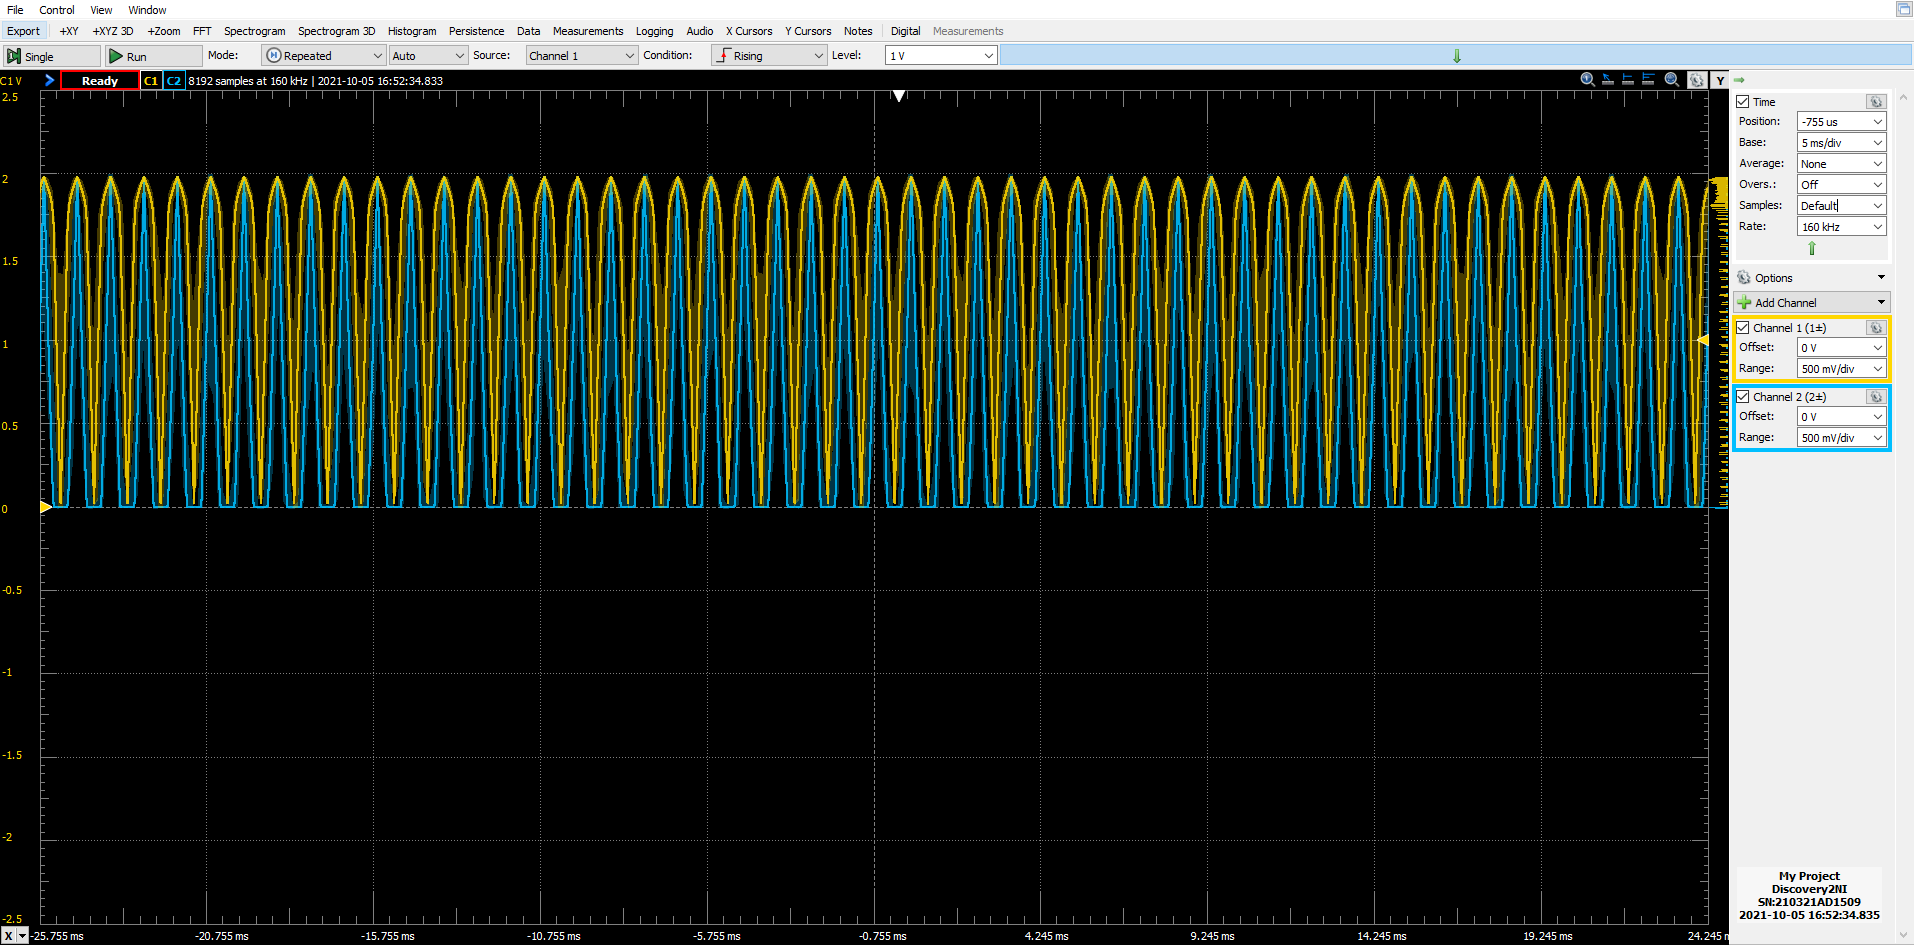
\includegraphics[scale=0.3]{trgdiode}
\caption{(4.e) Relazione tra trigger e segnale}
\end{figure}


\subsection*{4.f Misura tensione massima ai capi del diodo}
\par 
La tensione massima ai capi del diodo misurata con i cursori risulta essere
$V_{\mathrm{MAX}}= ( \exn \pm \exn ) \,\mathrm{V}$. La funzione di misura
automatica fornisce il valore $V_{\mathrm{AUTO}}= xx \,\mathrm{V}$

\vspace{0.5cm} 
\framebox(400,30){Inserire commento sulla accuratezza della misura.}



\section{Caratteristica del diodo}
\par

\subsection*{5.c Caratteristica del diodo}

\begin{figure}[h]
\centering
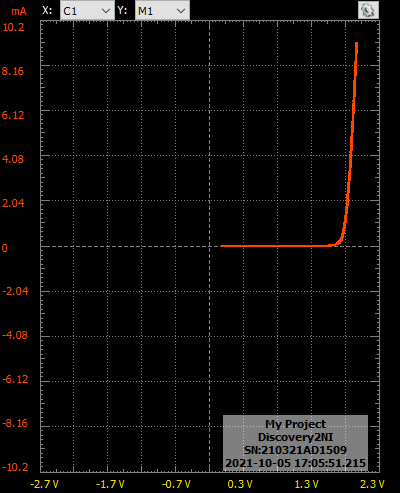
\includegraphics[scale=0.4]{shockley}
\caption{(5.c) Caratteristica corrente-tensione del diodo in modalit\`a XY}
\end{figure}

\subsection*{5.d Fit curva del diodo}
\par

\begin{figure}[h]
\centering
%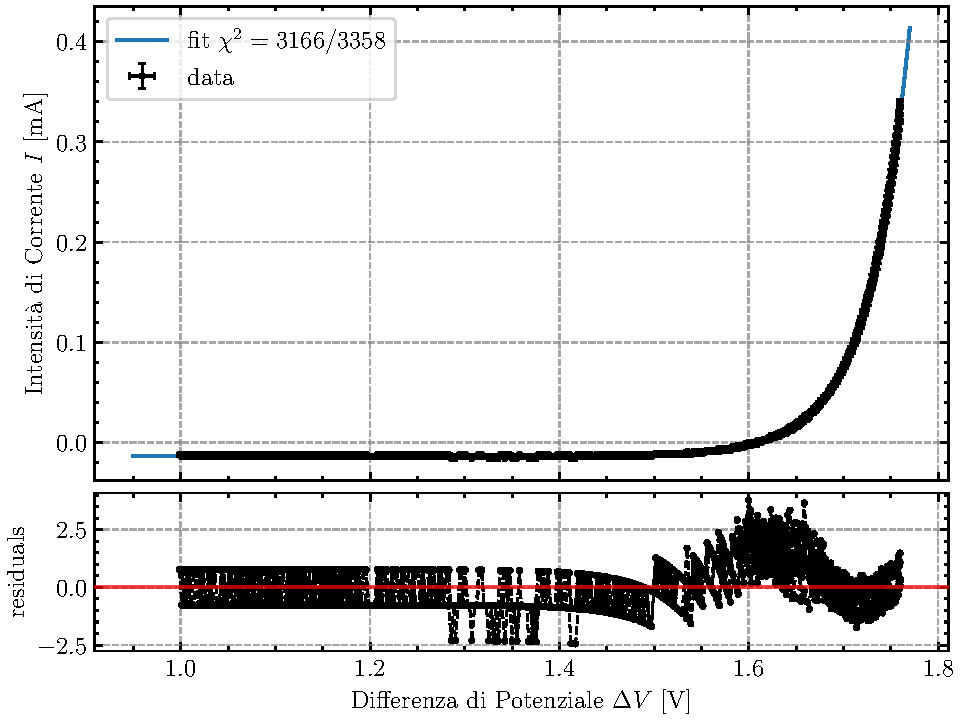
\includegraphics[scale=0.4]{ivfit}
\framebox(200,100){(2.b) Inserire il grafico $I_{D}$ vs. $V_{D}$ }
\caption{(2.b) Grafico $I_{D}$ vs. $V_{D}$ e fit all'equazione di Schockley}
\end{figure}



%=====================




\section{Partitore}

\subsection*{6.b Partitore con resistenze da 1k}


Si realizza un partitore con resistenze da $1 \,\mathrm{k}\Omega$.
Valori misurati con il multimetro: R1=$0.993 \pm \exn \,\mathrm{k}\Omega$,
R2=$0.993 \pm \exn \,\mathrm{k}\Omega$


\begin{table}[h]
\centering
\begin{tabular}{|c|c|c|c|c|c|}
\hline 
VIN& $\sigma$ VIN  &VOUT	 & $\sigma$ VOUT& VOUT/VIN & $\sigma$ VOUT/VIN \\
\hline 
\exn & \exn & \exn & \exn & \exn &\exn \\
\exn & \exn & \exn & \exn & \exn &\exn \\
\exn & \exn & \exn & \exn & \exn &\exn \\
\exn & \exn & \exn & \exn & \exn &\exn \\
\hline 
\end{tabular} 
\caption{(6.b) Partitore di tensione con resistenze da circa 1k. Tutte le
tensioni in V.\label{t:par1}}
\end{table}


\framebox(400,30){Inserire commento sul confronto tra valori misurati
ed attesi.}


\subsection*{6.d Partitore con resistenze da circa 1M}
\par
Si realizza un partitore con resistenze da $1 \,\mathrm{M}\Omega$.
Valori misurati con il multimetro: R1=$\exn \pm \exn \,\mathrm{M}\Omega$,
R2=$\exn \pm \exn \,\mathrm{M}\Omega$


\begin{table}[h]
\centering
\begin{tabular}{|c|c|c|c|c|c|}
\hline 
VIN& $\sigma$ VIN  &VOUT	 & $\sigma$ VOUT& VOUT/VIN & $\sigma$ VOUT/VIN \\
\hline 
\exn & \exn & \exn & \exn & \exn &\exn \\
\exn & \exn & \exn & \exn & \exn &\exn \\
\exn & \exn & \exn & \exn & \exn &\exn \\
\exn & \exn & \exn & \exn & \exn &\exn \\
\hline 
\end{tabular} 
\caption{(6.d) Partitore di tensione con resistenze da circa 1M.
Tutte le tensioni in V.\label{t:par2}}
\end{table}


\framebox(400,30){Inserire commento sul confronto tra valori misurati ed attesi.}



\subsection*{6.e Resistenza di ingresso del multimetro}
Usando il modello mostrato nella scheda si ottiene
\[ \frac{R_1}{R_T} =  \frac{V_{IN}}{V_{OUT}} - (1 +  \frac{R_1}{R_2} )
\]

Con i dati con resistenze da 1k si ottiene
\[ R_1/R_{IN} = \exn  \pm  \exn   \rightarrow  R_{IN} > \exn k\Omega
\]


Con i dati con resistenze da 1M si ottiene
\[ R_1/R_{IN} = \exn  \pm  \exn   \rightarrow  R_{IN} = (\exn \pm  \exn)  M\Omega
\]

\framebox(400,30){Inserire commento sulla sensibilit\`a sperimentale della misura.} 




\section{Misure di tempo e frequenza}

\subsection*{7.e Misure di frequenza}
Misure con onda sinusoidale
\begin{table}[h]
\centering
\begin{tabular}{|c|c|c|c|c|c|}
\hline 
Periodo T (s)& $\sigma$ T (s)  &Frequenza f (Hz) & $\sigma$ f (Hz) &
Misura oscilloscopio (Hz) & Differenza (Hz)\\
\hline 
\exn & \exn & \exn & \exn & \exn &\exn \\
\exn & \exn & \exn & \exn & \exn &\exn \\
\exn & \exn & \exn & \exn & \exn &\exn \\
\exn & \exn & \exn & \exn & \exn &\exn \\
\hline 
\end{tabular} 
\caption{(7.e) Misura di frequenza di onde sinusoidali e confronto con
misurazione interna dell'oscilloscopio }
\end{table}

\subsection*{7.f Misure di duty cyle}
Misure con onda quadra
\begin{table}[h]
\centering
\begin{tabular}{|c|c|c|c|c|c|}
\hline 
Periodo T (s)& $\sigma$ T (s) & Durata alto $t_H$ (s) & $\sigma$ $t_H$ (s)
& Duty cycle D(\%) & $\sigma$ D (\%) \\
\hline 
\exn & \exn & \exn & \exn & \exn &\exn \\
\exn & \exn & \exn & \exn & \exn &\exn \\
\exn & \exn & \exn & \exn & \exn &\exn \\
\exn & \exn & \exn & \exn & \exn &\exn \\
\hline 
\end{tabular} 
\caption{(7.f) Misura di duty cycle per onde quadre }
\end{table}


\subsection*{7.g Tempo di salita e di discesa}
Misure su onda quadra
\[
f = (\exn \pm \exn) \mathrm{MHz}, \quad
t_\mathrm{salita} = (35 \pm 6) \mathrm{ns},
t_\mathrm{discesa} = (37 \pm 6) \mathrm{ns},
\]

La misura è un po' balorda, visto che il tempo di salita/discesa è dello
stesso ordine di grandezza del periodo di campionamento $\nicefrac{1}{f_s} = \Delta t \approx 10 \si{\ns}$.
\framebox(400,30){Inserire commento su altre caratteristiche del segnale
ed eventualmente uno screenshot}

\section{Conclusioni e commenti finali}
\framebox(400,30){Inserire eventuali commenti e conclusioni finali}

\section*{Dichiarazione}
I firmatari di questa relazione dichiarano che il contenuto della relazione
\`e originale, con misure effettuate dai membri del gruppo, e che tutti i
firmatari hanno contribuito alla elaborazione della relazione stessa.

\end{document}